\documentclass[12pt,a4paper,openany,oneside]{report}
\usepackage[utf8]{vietnam}
\usepackage{amsmath, amsthm, amssymb,amsxtra,latexsym,amscd,graphpap,makeidx}
\usepackage{pgf,tikz}
\usepackage{mathrsfs}
\usetikzlibrary{arrows}
\usepackage{float}
 \usepackage{algorithm}
\usepackage{algpseudocode}
\usepackage{graphicx}
\usepackage{array,tabularx,longtable,multicol,indentfirst,fancyhdr}%
\usepackage[mathscr]{eucal}
\usepackage[top=3.5cm, bottom=3.0cm, left=3.5cm, right=2cm] {geometry}
\usepackage{fancybox}
%==================================  
\newtheorem{dl}{Định lý}[section]
\newtheorem{dn}[dl]{Định nghĩa} 
\newtheorem{bt}[dl]{Bài toán} 
\newtheorem{btp}[dl]{Bài tập} 
\newtheorem{bta}[dl]{Bài} 
\newtheorem{bai}[dl]{Bài}
\newtheorem{tc}[dl]{Tính chất} 
\newtheorem{md}[dl]{Mệnh đề} 
\newtheorem{bd}[dl]{Bổ đề} 
\newtheorem{hq}[dl]{Hệ quả} 
\newtheorem{nx}[dl]{Nhận xét} 
\newtheorem{cy}[dl]{Chú ý} 
\newtheorem{vd}[dl]{Ví dụ} 
\usepackage{hyperref}
\renewcommand{\chaptername}{Chương \chaptername}
\renewcommand\bibname{Tài liệu tham khảo}
%.....................................

\newcommand{\bpr}{\begin{proof}}
\newcommand{\epr}{\end{proof}}

 % package content table



%-----------------------------------------------
\def\en{\enskip}
\def\n{\noindent}
\def\m{\medskip}
\def\en{\enskip}
\def\m{\medskip}
\def\n{\noindent}
\def\Re{\mbox{Re }}
\def\Im{\mbox{Im }}
\def\hcm{\hfill $\square$\\}
\def\imotn{i = 1, 2, \ldots, n}
\def\ii{\item}


\def\N{\mathbb{N}}
\def\Z{\mathbb{Z}}
\def\R{\mathbb{R}}
\def\Q{\mathbb{Q}}
\def\C{\mathscr{C}}  
\def\K{\mathbb{K}}  
\def\F{\mathbb{F}}  
\def\L{\mathbb{L}} 
\DeclareMathOperator{\ord}{ord}

\allowdisplaybreaks
\newenvironment{giai}{\noindent{\em \textit{Giải}. }}{\hfill $\square$}

%%%%%%%%%%%%%%%%%%%%%%%%%%%% 
 
\makeatletter 
\renewcommand{\ps@plain}{
    \renewcommand{\@oddhead}{\hfil{\thepage}\hfil}
    \renewcommand{\@evenhead}{\@oddhead}
    \renewcommand{\@oddfoot}{\empty}
    \renewcommand{\@evenfoot}{\@oddfoot}   }
\makeatother
\pagestyle{fancy}
\fancyhf{}
\rhead{}
\chead{\normalsize  \thepage}
\lhead{\itshape {\nouppercase{}}}
\renewcommand{\headrulewidth}{0pt}





\begin{document}
	
	%Cô mới thêm vào đoạn này
	%========================================
	\pagestyle{fancy}
	\fancyhf{}
	\fancyhead[L]{Đồ án tốt nghiệp đại học} % Di chuyển header về bên trái
	\renewcommand{\headrulewidth}{0.4pt} % Gạch dưới header
	\fancyfoot[L]{Nguyễn Văn A - D19HTTT01 }
	\fancyfoot[R]{\roman{page}} % Số trang theo chữ số La mã ở bên phải của footer
	\renewcommand{\footrulewidth}{0.4pt} % Dòng kẻ trên footer
	
	\pagenumbering{gobble}
	
	%==============================================
%\pagenumbering{roman}

\newgeometry{top=2.0cm,bottom=3.0cm,left=3.0cm,right=2.8cm}
\setlength{\fboxrule}{1.5pt}
\thisfancypage{\setlength{\fboxsep}{10pt}\setlength{\shadowsize}{0pt}\doublebox}{}

\begin{titlepageaa}
\fontsize{14pt}{14pt}\selectfont \baselineskip 0.65cm
\thispagestyle{empty}
\begin{center}
{HỌC VIỆN CÔNG NGHỆ BƯU CHÍNH VIỄN THÔNG}\\
\textbf{\MakeUppercase{KHOA CÔNG NGHỆ THÔNG TIN I}}\\
\centerline{--------------------o0o--------------------}  
\end{center}
 

\begin{figure}[H]
	\begin{center}
		
\includegraphics[width=6cm]{./logo}
	\end{center}
\end{figure} 
 
 
\vspace{0.5cm}
\begin{center}
\textbf{\MakeUppercase{\LARGE \bf ĐỒ ÁN TỐT NGHIỆP ĐẠI HỌC}}\\ 
\end{center} 

\vspace{1cm}
\begin{center}
	Đề tài: 
	\textbf{\MakeUppercase{ \bf ``MỘT THUẬT TOÁN HIỆU QUẢ DỰA TRÊN CẠNH ĐỂ TỐI ƯU LỀ PHÂN LOẠI TRONG MẶT PHẲNG''}}\\ 
\end{center} 
\vspace{2cm}


\begin{tabular}{ll}
	{\textbf{\large{Giảng Viên Hướng Dẫn: }}} & {\textbf{\large{TS. Nguyễn Kiều Linh}}} \\
	{\textbf{\large{Sinh viên thực hiện:}}}  & {\textbf{\large{Nguyễn Văn A}}} \\
	{\textbf{\large{Mã sinh viên: }}}  & {\textbf{\large{BXXDCCNYYY}}} \\
	{\textbf{\large{Lớp:}}}   & {\textbf{\large{DXHTTTY}}}\\
	{\textbf{\large{Niên khóa:}}}   & {\textbf{\large{20xx-20xx}}}\\
	{\textbf{\large{Hệ đào tạo:}}}   & {\textbf{\large{Đại học chính quy}}}
\end{tabular}






\vfill
\begin{center}
{{\bf Hà Nội, 12/2023}}
\end{center}
\end{titlepage}

\newgeometry{top=2.0cm,bottom=3.0cm,left=3.0cm,right=2.8cm}
\setlength{\fboxrule}{1.5pt}
\thisfancypage{\setlength{\fboxsep}{10pt}\setlength{\shadowsize}{0pt}\doublebox}{}

\fontsize{14pt}{14pt}\selectfont \baselineskip 0.65cm
\thispagestyle{empty}
\begin{center}
	{HỌC VIỆN CÔNG NGHỆ BƯU CHÍNH VIỄN THÔNG}\\
	\textbf{\MakeUppercase{KHOA CÔNG NGHỆ THÔNG TIN I}}\\
	\centerline{--------------------o0o--------------------}  
\end{center}


\begin{figure}[H]
	\begin{center}
		
\includegraphics[width=6cm]{./logo}
	\end{center}
\end{figure} 



\vspace{0.5cm}
\begin{center}
	\textbf{\MakeUppercase{\LARGE \bf ĐỒ ÁN TỐT NGHIỆP ĐẠI HỌC}}\\ 
\end{center} 

\vspace{1cm}
\begin{center}
\textbf{Đề tài:}
	\textbf{\MakeUppercase{ \bf ``MỘT THUẬT TOÁN HIỆU QUẢ DỰA TRÊN CẠNH ĐỂ TỐI ƯU LỀ PHÂN LOẠI TRONG MẶT PHẲNG''}}\\ 
\end{center} 
\vspace{2cm}


\begin{tabular}{ll}
	{\textbf{\large{Giảng Viên Hướng Dẫn: }}} & {\large TS. Nguyễn Kiều Linh}\\
	{\textbf{\large{Sinh viên thực hiện:}}}  & {\large Nguyễn Văn A} \\
	{\textbf{\large{Mã sinh viên: }}}  & {\large BXXDCCNYYY} \\
	{\textbf{\large{Lớp:}}}   & {\large DXHTTTY}\\
	{\textbf{\large{Niên khóa:}}}   & {\large 20xx-20xx}\\
	{\textbf{\large{Hệ đào tạo:}}}   & {\large Đại học chính quy}
\end{tabular}


\vfill
\begin{center}
	{{\bf Hà Nội, 12/2023}}
\end{center}



%Cô mới thêm vào đoạn này
%========================================


%%%%%%%%%%%%%%%
\newgeometry{top=2.5cm,bottom=2cm,left=3cm,right=2cm} 
\thispagestyle{empty}
\begin{center}
	{\textbf{\Large{NHẬN XÉT CỦA GIẢNG VIÊN HƯỚNG DẪN}}}
\end{center}

\dotfill \vspace{0.25cm} \par
\dotfill \vspace{0.25cm} \par
\dotfill \vspace{0.25cm} \par
\dotfill \vspace{0.25cm} \par
\dotfill \vspace{0.25cm} \par
\dotfill \vspace{0.25cm} \par
\dotfill \vspace{0.25cm} \par
\dotfill \vspace{0.25cm} \par
\dotfill \vspace{0.25cm} \par
\dotfill \vspace{0.25cm} \par
\dotfill \vspace{0.25cm} \par
\dotfill \vspace{0.25cm} \par
\dotfill \vspace{0.25cm} \par
\dotfill \vspace{0.25cm} \par
\dotfill \vspace{0.25cm} \par
\dotfill \vspace{0.25cm} \par
\dotfill \vspace{0.25cm} \par
\dotfill \vspace{0.25cm} \par
\dotfill

\vspace{1cm}

{\textbf{\large{Điểm: }}} \hspace{1.0cm}\textbf{( Bằng chữ:}  \hspace{2.5cm}\textbf{)}  

\begin{flushright}
	Hà Nội, ngày \hspace{0.75cm} tháng \hspace{0.75cm} năm 20...\hspace{0.75cm}
	
	{\textbf{\large{Giảng viên hướng dẫn }}} \hspace{1cm} \textcolor{white}{.}
\end{flushright}



\newgeometry{top=2.5cm,bottom=2cm,left=3cm,right=2cm} 
\thispagestyle{empty}
\begin{center}
	{\textbf{\Large{NHẬN XÉT CỦA GIẢNG VIÊN PHẢN BIỆN}}}
\end{center}

\dotfill \vspace{0.25cm} \par
\dotfill \vspace{0.25cm} \par
\dotfill \vspace{0.25cm} \par
\dotfill \vspace{0.25cm} \par
\dotfill \vspace{0.25cm} \par
\dotfill \vspace{0.25cm} \par
\dotfill \vspace{0.25cm} \par
\dotfill \vspace{0.25cm} \par
\dotfill \vspace{0.25cm} \par
\dotfill \vspace{0.25cm} \par
\dotfill \vspace{0.25cm} \par
\dotfill \vspace{0.25cm} \par
\dotfill \vspace{0.25cm} \par
\dotfill \vspace{0.25cm} \par
\dotfill \vspace{0.25cm} \par
\dotfill \vspace{0.25cm} \par
\dotfill \vspace{0.25cm} \par
\dotfill \vspace{0.25cm} \par
\dotfill

\vspace{1cm}

{\textbf{\large{Điểm: }}} \hspace{1.0cm}\textbf{( Bằng chữ:}  \hspace{2.5cm}\textbf{)}  

\begin{flushright}
	Hà Nội, ngày \hspace{0.75cm} tháng \hspace{0.75cm} năm 20...\hspace{0.75cm}
	
	{\textbf{\large{Giảng viên phản biện }}} \hspace{1cm} \textcolor{white}{.}
\end{flushright}

%==============================================


\restoregeometry
\pagestyle{fancy}
\pagenumbering{roman}
\fontsize{13pt}{13pt}\selectfont \baselineskip 0.75cm 

\newpage
\thispagestyle{empty}
%\thispagestyle{fancy}
%\pagenumbering{roman}
%\vspace*{-2.5cm} % Thay đổi giá trị để điều chỉnh khoảng cách
% Tạo mục lục tự động
%\addcontentsline{toc}{chapter}{Mục lục}
\tableofcontents





%%%%%%%%%%%%%%%%%%%
\newpage
\begin{center}
	\Large{\textbf{LỜI CẢM ƠN}}\\
\end{center}
\vspace{1cm}
Đây là mục tùy chọn

...........................
\
 \\
 
 \
  \\
 \
  \\
 
\phantom{nnnnnnnnnnnnnnnnnnnnnnnnnnnnnnn}\  {\textit{Hà Nội, tháng ....  năm 20....}} \\
\phantom{nnnnnnnnnnnnnnnnnnnnnnnnnnnnnnnnnnnnnnnnn} {Sinh viên}\\
\phantom{nnnnnnnnnnnnnnnnnnnnnnnnnnnnnnnnnn} \\
\phantom{nnnnnnnnnnnnnnnnnnnnnnnnnnnnnnnnnn} \\ 
\phantom{nnnnnnnnnnnnnnnnnnnnnnnnnnnnnnnnnn} \\ 
\phantom{nnnnnnnnnnnnnnnnnnnnnnnnnnnnnnnnnnnnnnn}   {Nguyễn Văn A}


%%%%%%%%%%%%%%%%%%%%%%%%%%%%



\newpage 
\addcontentsline{toc}{chapter}{\bf  Danh sách hình vẽ} 

\listoffigures

%%%%%%%%%%%%%%%%%%%%%%%%%%%%

\newpage 
\addcontentsline{toc}{chapter}{\bf  Danh sách bảng} 
\listoftables

%%%%%%%%%%%%%%%%%%%%%%%%%%%%
	\newpage
{\addcontentsline{toc}{chapter}{Danh sách các ký hiệu và chữ viết tắt}}

\begin{center}
	{\LARGE
		{\bf Danh mục các ký hiệu và chữ viết tắt}}
\end{center}
\vspace{1.25cm}
{\fontsize{13}{13}\selectfont
	\begin{tabular}{ll}
		conv$(D)$ & bao lồi của tập hợp $D$\\
		$\partial ({\rm conv}(D))$ & biên của bao lồi conv$(D)$\\
		CH($D$) & tập các hình tròn cực biên của tập $D$\\
		$V_C$ & tập đỉnh của bao lồi conv($C$)\\
		$[p,q]$ & đoạn thẳng nối $p$ với $q$\\
		$pq$& đường thẳng đi qua $p$ và $q$\\
  .......... & ..................
	\end{tabular}
}


 
\newpage
\pagenumbering{arabic} 
\pagestyle{fancy} 

\chapter*{Mở đầu}
\addcontentsline{toc}{chapter}{\vspace*{-8pt}  Mở đầu} 


Hiện nay, công tác quản lý sinh viên bao gồm điểm danh sinh viên ra vào lớp học, xác thực danh tính sinh viên dự thi, kiểm soát sinh viên ra vào cổng trường, ... đều được thực hiện một cách thủ công như quẹt thẻ hoặc có người giám sát. Một sinh viên có thể điểm danh cho nhiều bạn vì hệ thống chỉ nhận diện được thông tin từ thẻ mà không nhận diện được người cầm thẻ, hoặc những người giám sát không thể so sánh, đối chiếu chính xác thông tin của tất cả sinh viên. Việc làm này với số lượng lớn sinh viên sẽ mất thời gian và thường khó đảm bảo sự chính xác cao.


Trong thời đại công nghệ thông tin ngày càng phát triển, mọi vấn đề đều được xử lý đơn giản và tối ưu hóa. Công nghệ nhận diện bằng sinh trắc học chính là chìa khóa cho những bài toán nhận diện, trong đó có nhận diện bằng khuôn mặt. Vì vậy, ứng dụng điểm danh trong lớp học sử dụng công nghệ điểm danh bằng khuôn mặt sẽ giúp cho việc điểm danh dễ dàng, nhanh chóng và chính xác hơn rất nhiều so với các phương pháp truyền thống.


Mục tiêu của đồ án là tìm hiểu, nghiên cứu các công nghệ nhận diện khuôn mặt và triển khai xây dựng ứng dụng cho bài toán điểm danh sử dụng công nghệ nhận diện khuôn mặt. Ngoài ra, đồ án còn tìm hiểu và phát triển khả năng chống giả mạo cho ứng dụng nhận diện khuôn mặt.


Trong đồ án em sẽ tập trung trình bày một số nội dung chính như sau:

\textbf{Chương 1: Tổng quan về các tác vụ cho bài toán nhận dạng giọng nói:}
Nội dung chương 1 sẽ khái quát các vấn đề và phương pháp nhận dạng giọng nói, khảo sát về các phương pháp học máy đang được sử dụng cho ba nhiệm vụ con, và trình bày về phạm vi của đồ án.


\textbf{Chương 2: Nhận dạng giọng nói bằng mô hình chưng cất và học đa tác vụ:}
Nội dung của chương 2 sẽ giới thiệu kiến thức cơ bản về trí tuệ nhân tạo và các mạng thần kinh học sâu cũng như các bước xây dựng mô hình chưng cất gọn nhẹ đa tác vụ dựa trên cơ chế chú ý và các kỹ thuật như cắt tỉa mô hình và chưng cất tri thức.


\textbf{Chương 3: Thực nghiệm và kết quả:}
Nội dung của chương 3 trình bày quá trình thu thập dữ liệu, mô tả phương pháp thực nghiệm và đánh giá mô hình chưng cất ứng dụng vào nhận dạng giọng nói và trình bày các kết quả của quá trình thực nghiệm.


\textbf{Chương 4: Tổng kết:}
Tổng kết bài toán, tóm tắt những kết quả đã đạt được và còn chưa đạt được. Từ đó đề xuất mục tiêu hướng tới cũng như hướng nghiên cứu, phát triển tiếp theo.


% ===================================================


\chapter{Kiến thức chuẩn bị}
%\addcontentsline{toc}{chapter}{} 

Chương 1 trình bày phát biểu và chứng minh định lý Fermat nhỏ, định lý Euler. Trình bày khái niệm và cách giải phương trình đồng dư tuyến tính, hệ phương trình đồng dư tuyến tính (định lý thặng dư Trung Hoa). Các kiến thức ở chương này giúp việc trình bày ở chương sau được hệ thống và dễ theo dõi hơn.



\section{Thuật toán Quickhull}
Trong các thuật toán tìm bao lồi thì thuật toán Quickhull \cite{David-2002, Rourke-1998} được biết đến là một thuật toán hiệu quả có độ phức tạp tính toán trung bình là $O(n \log n)$ nhưng trong trường hợp xấu nhất thì độ phức tạp là $O(n^2)$, trong đó $n$ là số điểm của tập điểm đầu vào của thuật toán. Độ phức tạp của thuật toán Quickhull tương tự như thuật toán Quicksort - một thuật toán sắp xếp hiệu quả dựa trên việc phân chia mảng dữ liệu thành các nhóm phần tử nhỏ hơn và thuật toán này chạy trong thực tế nhanh hơn rất nhiều so với trường hợp xấu nhất. Để giải thích cho điều này, V. Damerow và C. Sohler đã đánh giá thành công số điểm cực biên của một tập hợp theo nghĩa Smoothed analysis \cite{Damerow-2004}. Từ đó có thể đánh giá độ phức tạp tính toán của thuật toán Quickhulll theo nghĩa này trong hai trường hợp là:
\begin{itemize}
	\item Nhiễu ngẫu nhiên của tập điểm được chọn từ phân bố chuẩn $N(0, \delta)$: 
	O$\left( n \left(\dfrac{1}{\delta} \right)^2 \log^2 n\right) $.
	\item Nhiễu ngẫu nhiên được chọn từ phân bố đều trong hình vuông kích thước $2 \epsilon$: 
	O$\left( n \left(\dfrac{n \log n}{\epsilon} \right)^{2/3}\right). $
\end{itemize}

Bài toán tìm bao lồi có ứng dụng rất quan trọng trong lĩnh vực nhận dạng. Các ứng dụng phổ biến của nhận dạng trong thực tế là nhận dạng tiếng nói tự động, phân loại văn bản thành nhiều loại khác nhau (ví dụ những thư điện tử spam/non-spam), nhận dạng tự động các mã bưu điện viết tay trên các bao thư, hay hệ thống nhận dạng mặt người, nhận dạng biển số xe, v.v\ldots Sau đây ta xét một ứng dụng cụ thể của bài toán tìm bao lồi trong nhận dạng biển số xe. 
\begin{figure}[ht!]
	\begin{center}
		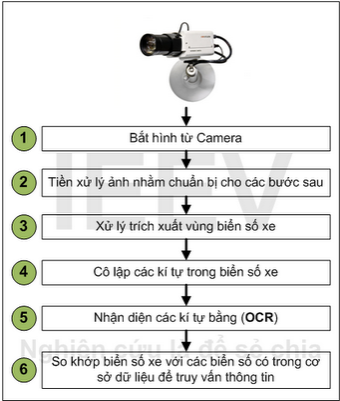
\includegraphics[width=200px]{./nhandang1.PNG}
		\caption{Quy trình tự động nhận dạng biển số xe.}
		\label{fig_dhandang1}
	\end{center}
\end{figure} 

\section{Sơ lược về ............ }
\begin{dn}\rm {\it Phương trình đồng dư đại số bậc $n$} là một đồng dư thức có dạng
\begin{align} \label{ptdd}
f(x)= a_0x^n + a_1x^{n-1} + \ldots + a_n \equiv 0\pmod{m}
\end{align}
trong đó $x$ là ẩn, $a_i \in \mathbb{Z}$ (với $i = 1, 2, \ldots, n$) và $a_0\not\equiv 0\pmod m$.
\end{dn} 
\begin{cy}\rm (i) Giải phương trình (\ref{ptdd}) là tìm tất cả các giá trị nguyên của $x$ thoả mãn đồng dư thức (\ref{ptdd}). Nếu $x = x_0$ thoả mãn phương trình (\ref{ptdd}) thì mọi số $x \equiv x_0\pmod{m}$ đều thoả mãn (\ref{ptdd}); trong trường hợp này tập hợp $\{x\in\Z\mid x\equiv x_0\pmod m\}$ được gọi là một {\it nghiệm} của phương trình đồng dư (\ref{ptdd}), kí hiệu là $\overline{x_0}$ hoặc $x\equiv x_0\pmod m$.\par
\item (ii) Số nghiệm của phương trình (\ref{ptdd}) là số các phần tử trong một hệ thặng dư đầy đủ theo modulo $m$ mà thỏa mãn (\ref{ptdd}).\par
\item (iii) Hai phương trình đồng dư được gọi là tương đương nếu tập hợp các số nguyên thỏa mãn các phương trình đó là trùng nhau.
\end{cy}

\begin{vd} \rm Xét phương trình $x^2 \equiv 1 \pmod{5}$.
\end{vd}

\begin{giai} Ta thấy trong các số 0, 1, 2, 3, 4 của hệ thặng dư không âm bé nhất theo modulo 5, có hai số 1 và 4 thỏa mãn phương trình đã cho. Vậy phương trình có hai nghiệm là $x \equiv 1 \pmod{5}$ và $x \equiv 4 \pmod{5}$.
\end{giai}

\begin{vd} \rm Giải phương trình đồng dư $x^4 + 7x + 4 \equiv 0\pmod{9}$.
\end{vd}
\begin{giai} Dễ thấy phương trình $x^4 + 7x + 4 \equiv 0\pmod{3}$ có nghiệm là $x \equiv 1\pmod{3}$ (hay $x = 3t +1$ với $t\in\Z$). Thay $x$ vào phương trình cần giải và bỏ đi những số hạng chia hết cho 9 ta được
	\begin{align*}
	&6t + 3  \equiv 0\pmod{9}\\
	\Leftrightarrow \ & 2t + 1  \equiv 0\pmod{3}\\
	\Leftrightarrow \ & t \equiv 1\pmod{3}\\
		\Leftrightarrow \ & t = 3k +1.
	\end{align*}
Vậy phương trình có nghiệm là $x = 3(3k+1) + 1$ hay $x \equiv 4\pmod{9}$.
\end{giai}

 \begin{dn} \rm Phương trình đồng dư $ax \equiv b \pmod{m}$ được gọi là {\it phương trình đồng dư tuyến tính} với $a, b, m$ là các số nguyên đã biết. Khi đó $x\equiv x_0\pmod m$ là một nghiệm của phương trình khi và chỉ khi $ax_0 \equiv b\pmod{m}$.
\end{dn}





\chapter{Ứng dụng .................}

Chương này trình bày định nghĩa và các tính chất của thặng dư bậc hai: cách tính thặng dư bằng định nghĩa, cách tính thặng dư thông qua ký hiệu Legendre, cách tính thông qua luật thuận nghịch bậc hai. Sau đó ứng dụng thặng dư bậc hai và luật thuận nghịch bậc hai để tính toán và giải một số bài toán chứng minh, tìm căn nguyên thủy, kiểm tra tính nguyên tố.  

\section{Thặng dư bậc hai và ứng dụng}
Thặng dư bậc hai đóng vai trò rất quan trọng trong lý thuyết số. Chẳng hạn, thuật toán phân tích số nguyên ra thừa số nguyên tố. Ngoài ra thặng dư bậc hai cũng ứng dụng lớn trong mật mã cũng như trong các giao thức mã hóa.... Ở đây ta xét ứng dụng liên quan đến giải phương trình đồng dư bậc hai trong lý thuyết và thực hành.
 
\subsection{Phương trình đồng dư bậc hai..........}
Xét phương trình đồng dư bậc hai theo modulo nguyên tố (theo tài liệu \cite{K2007}).
\begin{align}\label{pt7.1}
Ax^2 + Bx + C \equiv 0 \pmod{p},
\end{align}
trong đó $p$ nguyên tố lẻ và $A, B, C \in \mathbb{Z}$ với $p\nmid A$. (Nếu $p\mid A$ thì quay về phương trình tuyến tính). Vì $p$ nguyên tố lẻ và $p\nmid A$, nên $p\nmid 4A$. Ta nhân hai vế của phương trình với $4A$ ta được
\begin{equation}\label{pt7.2}
4A(Ax^2+Bx+C)\equiv 0\pmod p.
\end{equation}
Nhưng ta có 
\begin{align*}
4A(Ax^2+Bx+C)&=4A^2x^2+4ABx+4AC\\
&=(2Ax+B)^2-(B^2-4AC).
\end{align*}
Do đó đồng dư thức (\ref{pt7.2}) được viết lại thành
\begin{align*}
(2Ax+B)^2\equiv (B^2-4AC)\pmod p
\end{align*}
nó có dạng 
\begin{align}\label{pt7.3}
y^2\equiv a\pmod p
\end{align}
 trong đó $y=2Ax+B$ và $a=B^2-4AC$.\par 
Nếu phương trình $y^2\equiv a\pmod p$ có nghiệm, thì ta suy ra phương trình $2Ax+B=y$ có nghiệm $x$ modulo $p$ (vì $(2A,p)=1$). Do đó phương trình (\ref{pt7.1}) có nghiệm nếu và chỉ nếu phương trình (\ref{pt7.3}) có nghiệm.\par

Ví dụ sau sẽ minh họa điều này.

	{\fontsize{12pt}{12pt}\selectfont \baselineskip 0.65cm
	\renewcommand{\baselinestretch}{1.0}	
	\begin{algorithm}[ht!]
		
		\floatname{algorithm}{Thuật toán}
		\caption{\textsc{Thuật toán tìm bao lồi dưới} $\hbox{conv}_L(P)$}  \label{al-blduoi}
		\textbf{Đầu vào: }Cho $P=\{p_i=(x_i,y_i,z_i)\in \mathbb{R}^3,\ i=1,\dots,n\}, n\ge 3$.\\
		\textbf{Đầu ra:} Tập ${\cal Q}$ tất cả các mặt dưới của $\hbox{conv}_L(P)$.
		
		\begin{algorithmic}[1]
			
			
			\State Tìm cạnh đầu tiên $e_0$ của $\hbox{conv}_L(P)$. 
			\State Xét hàng đợi ${\cal Q}:=\emptyset$ và tập ${\cal E}_L(P):=\emptyset$.
			
			\State Gọi {\bf LFRes}($e, P$) để nhận được một mặt dưới $F_e$ qua $e_0$. Đẩy các cạnh của $F_e$  trừ $e_0$ vào trong ${\cal E}_L(P)$. Đẩy $F_e$ vào trong tập ${\cal Q}$.
			
			\State  {\bf while} $({\cal Q}\ne\emptyset)$ {\bf do}
			
			\State 
			\quad \quad Lấy $F_e$ từ phía trên của  ${\cal Q}$.
			
			\State 	\quad \quad \quad \quad $T:=$ tập các cạnh $F_e$.
			
			\State 	\quad \quad \quad \quad {\bf for each} $e \in T\cap  {\cal E}_L(P)$ {\bf do}
			
			\State 
			\quad \quad\quad \quad\quad \quad Gọi {\bf LFRes}($e, P$) để nhận được mặt $F'_e$ có chung cạnh $e$ với $F_e$. \hspace*{2.5cm}Đưa vào ${\cal E}_L(P)$ tất cả các cạnh $e' \ne e_0$ của $F'_e$ chưa xuất hiện trong \hspace*{2.5cm} ${\cal E}_L(P)$ và xoá các cạnh đã xuất hiện trong ${\cal E}_L(P)$. Đẩy $F'_e$ vào ${\cal Q}$.
		
			
		\end{algorithmic}
	\end{algorithm}
}

	\chapter{Một số kết quả tính toán }
Trong nội dung này chúng tôi thử nghiệm số cho thuật toán trong \cite{An-Giang} và thuật toán vừa được trình bày ở mục trước để so sánh tốc độ của chúng. Các thuật toán này được thực thi bởi chương trình C và chạy trên PC Core i5 1.6 GHz 3M với 4 GB RAM.  

Dưới đây Bảng \ref{tab:51} minh họa thời gian chạy (đơn vị tính bằng giây) của thuật toán tính bao lồi dưới được giới thiệu bởi P. T. An và D. T. Giang trong \cite{An-Giang} và Thuật toán \ref{al-matduoi} sử dụng kỹ thuật hạn chế của chúng tôi. Cột cuối cùng liệt kê tỉ lệ tăng tốc của thuật toán của chúng tôi so với thuật toán trong \cite{An-Giang}. Dữ liệu đầu vào của các thuật toán là các tập điểm được tạo trên bề mặt một paraboloid (tất cả các điểm đều là đỉnh của bao lồi và bao lồi dưới) có dạng $P = \{p_i = (x_i, y_i, z_i): x_i, y_i, z_i \in \mathbb{R}, z_i = x_i^2 + y_i^2, i = 1, \ldots, n\} \subset \mathbb{R}^3,$ trong đó tập $\{(x_i, y_i), x_i, y_i \in R, i = 1, \ldots , n \}$ được chọn ngẫu nhiên từ phân bố đều trong hình vuông cỡ 200 $\times$ 200. 

{\fontsize{12pt}{12pt}\selectfont \baselineskip 0.65cm
	\renewcommand{\baselinestretch}{1}
	\begin{table}[ht!]
		\begin{center}
			\caption{Thời gian chạy tính bao lồi dưới (đơn vị: giây).}
			\label{tab:51}
			\begin{tabular}{cccc}
				\hline
				{Đầu vào} &{Thuật toán trong} \cite{An-Giang} & {Thuật toán} \ref{al-blduoi}& Tỉ số thăng tốc\\
				\hline
				1.000 & 0,136& 0,061&2,23\\ 
				2.000 & 0,454& 0,248 &1,83\\  
				5.000 & 2,684& 1,500 &1,79\\  
				7.000 & 7,014& 3,129 &2,24\\ 
				11.000  & 14,321& 8,484 &1,69\\ 
				17.000  & 41,307& 24,666 &1,67\\ 
				20.000 & 63,197& 37,332 &1,69\\  
				22.000 & 70,866& 40,235 & 1,76\\ 
				30.000 & 153,240& 96,738 &1,58\\ 
				35.000& 200,496& 125,490& 1,60\\ \hline	
			\end{tabular}	
		\end{center}
	\end{table}	
}







\chapter*{{Kết luận}}
\addcontentsline{toc}{chapter}{\vspace*{-8pt} Kết luận}

 Trong quá trình thực tập, em đã có cơ hội làm quen một môi trường làm việc mới. Em đã tính lũy những kinh nghiệm về kiến thức trong công việc cũng như các kinh nghiệm về kỹ năng mềm.
 
 Em được rèn luyện kĩ năng giải quyết công việc theo từng giai đoạn, cố gắng hoàn thành công việc trong thời gian cho phép, mạnh dạn trao đổi và chia sẻ kiến thức. Đồng thời cũng bồi dưỡng thêm rất nhiều kiến thức ngoài các kiến thức đã học trên trường.
 




\begin{thebibliography}{30}
\addcontentsline{toc}{chapter}{\vspace*{-8pt} Tài liệu tham khảo}
	
\subsection*{Tiếng Việt}

\bibitem{G2016} Vũ Thị Gái (2016), \textit{Luật thuận nghịch bậc hai và điểm nguyên}, trường Đại học Khoa học, Đại học Thái Nguyên.

\bibitem{D2005} Nguyễn Tiến Hùng (2016), \textit{Luật thuận nghịch bậc hai và hoán vị}, trường Đại học Khoa học, Đại học Thái Nguyên.


\bibitem{K1997} Hà Huy Khoái (1997), \textit{Nhập môn số học thuật toán}, Nhà xuất bản Khoa học Kỹ thuật.

\bibitem{LDT} Lại Đức Thịnh (1977), {\it Giáo trình số học}, Nhà xuất bản Giáo dục.
	
\subsection*{Tiếng Anh}
	\bibitem{An-Giang} P. T. An and D. T. Giang (2015), ``A direct method for determining the lower convex hull of a finite point set in 3D'', Advances in Intelligent Systems and Computing, \textit{Springer}, Proceedings of 3rd International Conference on Computer Science, Applied Mathematics and Applications (ICCSAMA, May 11-13, Metz, France) \textbf{358},  pp. 15--26.


\bibitem{Damerow-2004} V. Damerow and C. Sohler (2004), ``Extreme points under random noise'', \textit{Eropean Symposium on Algorithms} {\bf 3221}, pp. 264--274.
\bibitem{David-2002}  M. M. David (2002), \textit{Computation geometry}, Department of Computer Science.

\bibitem{Rourke-1998} J. O' Rourke (1998), \textit{Computational geometry in C}, 2nd edition, Cambridge University Press, Cambridge. 
	
\end{thebibliography} 
\end{document}
 
